\documentclass[11pt,a4paper]{article}
\usepackage[T1]{fontenc}
\usepackage[utf8]{inputenc}
\usepackage[french]{babel}
\usepackage{lmodern}
\usepackage{amsmath,amssymb}
\usepackage[margin=2.5cm]{geometry}
\usepackage{booktabs}
\usepackage{graphicx}
\usepackage{enumitem}
\usepackage{xcolor}
\usepackage{hyperref}
\hypersetup{colorlinks=true,linkcolor=blue!50!black}

\newcommand{\NW}{\mathrm{NW}}
\newcommand{\code}[1]{\texttt{#1}}

\title{Note 07 — Mini-protocole X1 : la règle de maximisation du revenu\\
\large Extension post-M3 du programme (workspace \code{m3\_credit\_soc})}
\author{Agent de recherche M3}
\date{6 juillet 2026}

\begin{document}
\maketitle

\begin{abstract}
Que devient M3 si la règle comportementale des entités n'est plus « se
rapprocher de la taille optimale » mais « maximiser son revenu net » ?
Formellement : l'emprunteuse vise $K^*(r)$ (rendement marginal $=$ taux
d'intérêt) au lieu de $K^*(r+\delta)$ (rendement marginal $=$ coût complet,
dépréciation incluse) — la maximisation \emph{myope du flux de revenu}
ignore l'érosion du stock. Résultat central, robuste sur les six cellules
testées : \textbf{ce seul changement de règle transforme le régime — le
service de la dette passe de $1{,}5\,\%$ à $6$--$14\,\%$ de la production,
les défauts de liquidité deviennent systématiques (jusqu'à un quart des
faillites à $s{=}0{,}9$), l'espérance de vie est divisée par $\sim 8$, la
population par $\sim 8$, le Gini de $\NW$ monte de $0{,}56$ à
$0{,}62$--$0{,}69$ et la part des intérêts dans le revenu du top 1\,\%
atteint $9$--$22\,\%$}. La conclusion « le crédit est distributionnellement
neutre » de M2 et M3 est donc \emph{conditionnelle à la règle
comportementale} : avec des agents myopes au revenu, le crédit devient
distributionnellement actif. En revanche, toujours aucune signature SOC :
même sous levier lourd, les avalanches causales restent sous-Poisson.
\end{abstract}

\section{La règle, et un résultat analytique}

Dans M3 (rapport 02 §3, phase 6), le volume d'un prêt est
$q = \min(A_\ell,\, K^*(\rho) - K_b)$ avec $\rho = r + \delta$ : l'emprunteuse
s'endette jusqu'au point où le rendement marginal couvre le \emph{coût
complet} du capital — c'est l'objectif « richesse soutenable ». X1 remplace
$\rho = r + \delta$ par $\rho = r$ : l'entité emprunte tant que sa production
marginale couvre l'intérêt, sans internaliser la dépréciation (qui érode la
richesse, pas le revenu). Un seul champ de configuration change
(\code{objective="income"}), rien d'autre.

Avec le taux en moyenne géométrique $r = \sqrt{r_\ell r_b}$ et
$r_x = \alpha/(2\sqrt{K_x})$, la cible devient :
\[
K^*(r) \;=\; \frac{\alpha^2}{4\,r_\ell r_b} \;=\; \sqrt{K_\ell K_b}\,.
\]
\textbf{La règle de revenu fait du crédit une dynamique d'égalisation des
capitaux} : chaque rencontre pousse l'emprunteuse vers la moyenne géométrique
des deux tailles (dans la limite de la liquidité prêtable), contre une cible
fixe $K^*(r+\delta) \approx 23$ sous la règle richesse. Le levier est
mécaniquement démultiplié. Identité vérifiée par test unitaire
(\code{test\_market\_income\_objective}, 51 tests verts).

\section{Protocole}

Statut : protocole dédié post-M3, défini avant exécution dans
\code{experiments/m3/run\_income\_protocol.py}, mais \emph{non}
pré-enregistré au sens du rapport 02 (pas de critères d'acceptation gelés) —
les comparaisons ci-dessous sont descriptives. Cellules ($3$ seeds
$\times\ T{=}2000$ chacune) : baseline X1 ; $\sigma \in \{0{,}20, 0{,}30\}$ ;
$k \in \{3, 12\}$ ; $s = 0{,}9$. \textbf{L'ablation sans crédit de X1 est
identiquement l'ablation B de M3} (l'objectif n'intervient que dans le
marché, inerte quand \code{credit=False}) : elle n'est pas relancée, les
10 seeds de B servent de référence. Toute différence X1$\,$vs$\,$B est donc
médiée par le crédit, et toute différence X1$\,$vs$\,$A isole l'effet de la
règle.

\section{Résultats}

\begin{center}
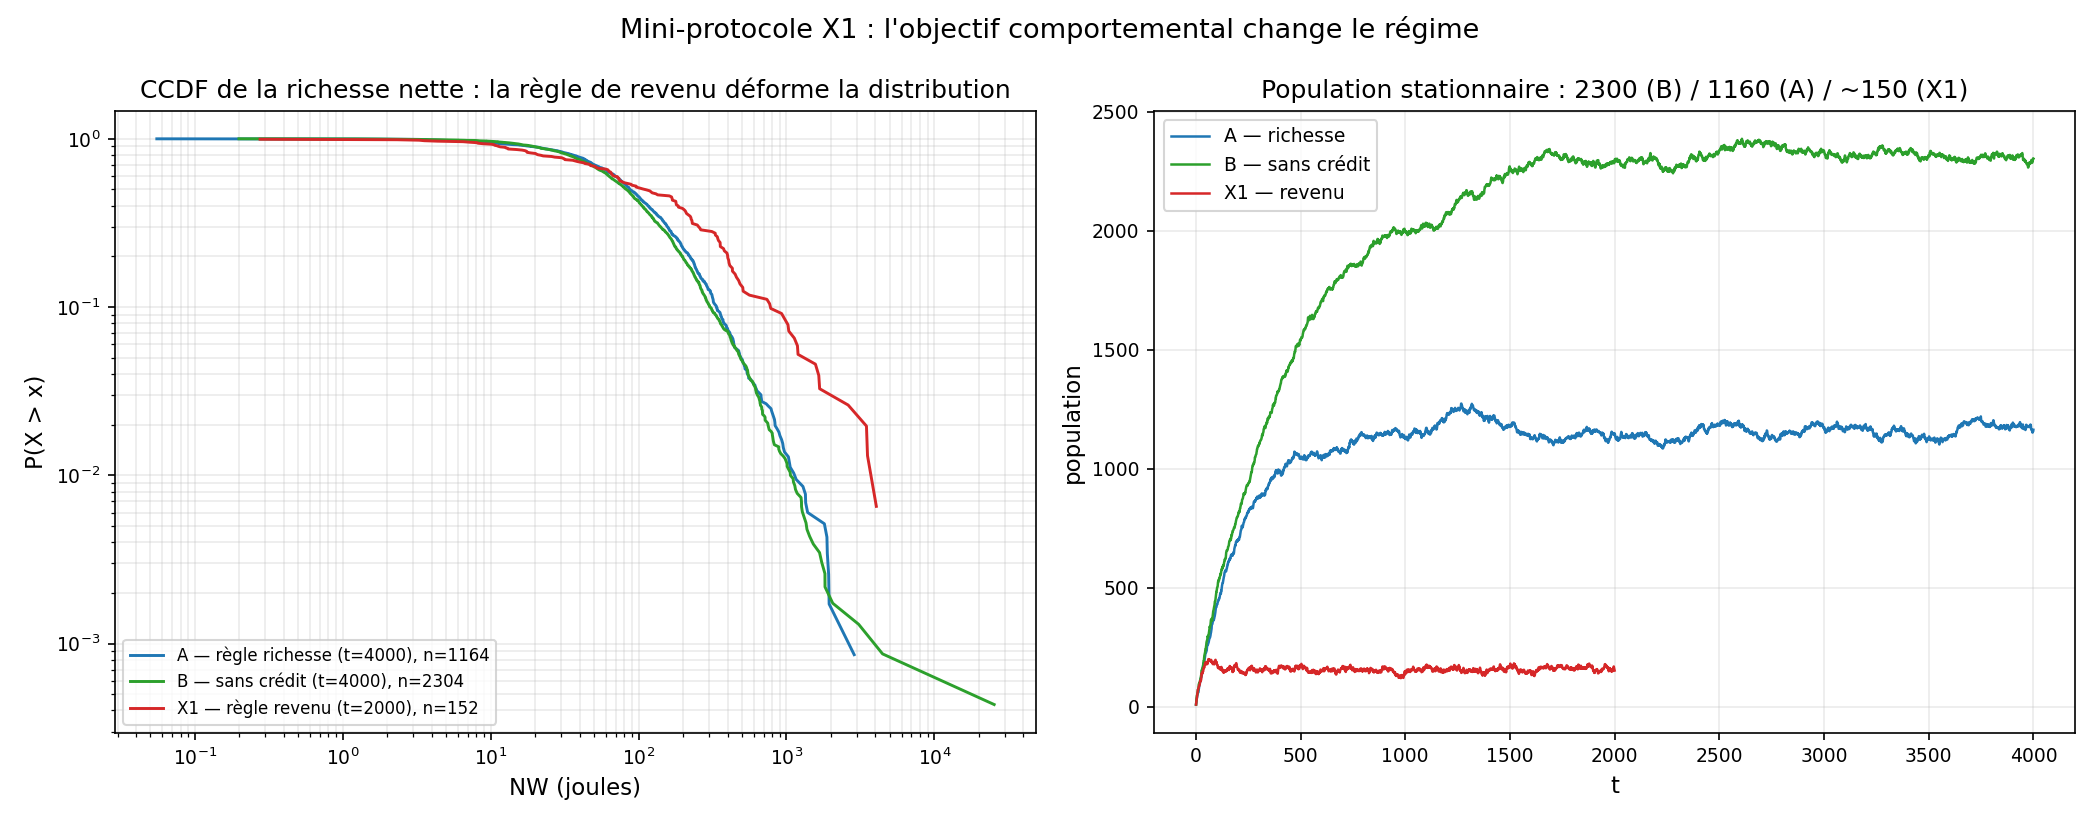
\includegraphics[width=\textwidth]{figures/x1_comparison.png}
\end{center}

\begin{center}
\small
\begin{tabular}{lccccccc}
\toprule
Cellule & pop & morts/nais. & $\frac{\text{intérêts}}{\text{production}}$ &
\% racines liquidité & aval. (v/m ; max) & $\alpha_{\NW}$ & Gini($\NW$) \\
\midrule
A (référence M3)   & 1160 & 1,00 & 1,5\,\%  & 0\,\%    & 0,07 ; 7 & 2,69 & 0,57 \\
B (sans crédit)    & 2330 & 1,00 & ---      & ---      & --- ; 1  & 2,69 & 0,56 \\
\midrule
X1 base            & 151  & 1,00 & 12,4\,\% & 1,4\,\%  & 0,01 ; 4 & 2,37 & 0,69 \\
X1 $\sigma{=}0{,}20$ & 202 & 1,00 & 13,4\,\% & 5,1\,\%  & 0,01 ; 5 & 2,53 & 0,63 \\
X1 $\sigma{=}0{,}30$ & 129 & 1,00 & 10,3\,\% & 0,3\,\%  & 0,01 ; 4 & 2,71 & 0,63 \\
X1 $k{=}3$         & 153  & 1,00 & 14,3\,\% & 2,9\,\%  & 0,11 ; 8 & 2,37 & 0,67 \\
X1 $k{=}12$        & 175  & 1,00 & 9,7\,\%  & 0,7\,\%  & 0,00 ; 3 & 2,55 & 0,65 \\
X1 $s{=}0{,}9$     & 195  & 1,00 & 5,6\,\%  & \textbf{24,2\,\%} & 0,02 ; 4 & 2,63 & 0,62 \\
\bottomrule
\end{tabular}
\end{center}

\begin{enumerate}[leftmargin=1.6em, itemsep=3pt]
\item \textbf{Le canal de fragilité nominale, inerte dans tout M3, devient
  structurel.} Les défauts de liquidité (entités solvables mais illiquides)
  apparaissent dans toutes les cellules, et représentent \emph{un quart des
  faillites} à $s = 0{,}9$ (afflux de liquidité minimal $\times$ service
  lourd). Le service de la dette atteint $6$--$14\,\%$ de la production
  ($\times 4$ à $\times 10$ vs M3).
\item \textbf{Le régime démographique s'effondre et se re-stabilise très
  bas} : population $129$--$220$ (vs $1160$), morts/naissances $= 1{,}00$
  partout, espérance de vie $\approx 15$ pas (vs $116$). Fait notable : à
  $\sigma = 0{,}20$, qui \emph{divergeait} sous la règle richesse
  ($N \approx 6000$ et croissant), X1 est borné — la mortalité par
  sur-levier remplace la mortalité par chocs et élargit la fenêtre
  d'existence du régime.
\item \textbf{Le crédit devient distributionnellement actif.} Gini($\NW$)
  $= 0{,}62$--$0{,}69$ contre $0{,}56$--$0{,}57$ pour A \emph{et} B
  (écart $\gg$ variabilité inter-seed) ; la CCDF de $\NW$ se déforme
  visiblement (figure) ; la part des intérêts dans le revenu du top 1\,\%
  atteint $9$--$22\,\%$ (vs $2{,}7$--$4{,}7\,\%$) : de vrais revenus de
  rentière apparaissent. La conclusion centrale de M2/M3 — « le crédit ne
  change pas les distributions » — est donc \emph{conditionnelle à la règle
  comportementale} : elle vaut pour des agentes qui internalisent le coût
  complet du capital, pas pour des maximisatrices myopes de revenu.
  Réserve de puissance : avec $n \approx 150$ par instantané, les familles
  de corps ne sont plus identifiables de façon stable (lognormale, gamma et
  Fisk alternent selon les seeds) et les $\alpha$ de queue portent des IC
  larges — les verdicts fermes portent sur le Gini, la CCDF, la
  financiarisation et les canaux de mortalité, pas sur les familles.
\item \textbf{Toujours pas de SOC.} Malgré le levier lourd et les défauts
  de liquidité, les avalanches causales restent sous-Poisson dans toutes
  les cellules (var/moy $\le 0{,}11$, max $8$). L'hypothèse
  accumulation--relaxation ne tient pas davantage sous sur-endettement
  myope : troisième réfutation de régime après M3-baseline et les chocs
  corrélés.
\end{enumerate}

\section{Lecture d'ensemble et suite}

X1 est la première modification du programme qui rende le crédit
\emph{distributionnellement} actif — et elle le fait par le canal exact que
M3 avait construit puis trouvé dormant : l'asymétrie nominal/réel
(obligations exigibles en liquidité contre actif illiquide), qui ne mord que
si le service de la dette est lourd. La leçon pour M4 est directe : le
paramètre décisif n'est pas l'architecture comptable du crédit mais la
\emph{règle d'endettement} des agentes ; combinée au plancher endogène
découvert en H ($d_0$ remplacé par une dette de subsistance), la règle de
revenu fournit le régime à levier élevé dans lequel tester proprement la
thèse SOC — qui, à ce stade, a résisté à trois régimes très différents sans
jamais montrer de signature critique.

\section{Traçabilité}

Champ \code{objective} dans \code{config.py} (défaut \code{"wealth"}
inchangé — la baseline M3 et R1 sont intacts, 51 tests verts) ; 18 runs
archivés \code{x1\_*} avec \code{validation.json} ; figures par run dans
l'explorateur web (groupe X1) ; budget : $\approx 0{,}1$ h de simulation
(cumul programme : $20{,}5$ h / 48).

\end{document}
